\chapter{Développement d'application}

Comme expliqué dans l'introduction chapitre ~\ref{chap:intro} le premier objectif du stage était le développement d'applications de réalité augmentée spatiale. Il était important pour commencer, d'évaluer les possibilités mais aussi les contraintes qu'offrait le kit de développement.
Ainsi un travail d'analyse et de critique de l'API à été effectué en parallèle du développement d'applications.

\section{ReARTable}
\label{sec:reartable}
D'après le contexte et le public ciblé par l'entreprise, il m'a paru intéressant de développer une démonstration a but à la fois ludique et éducatif. J'ai donc choisit de recréer une Reactable\cite{reactable} proposé par la société du même nom en réalité augmentée spatiale.

La Reactable est un instrument de musique électronique permettant la génération de son en direct développé depuis 2003. Présenté sous forme d'une table interactive, le son est généré via des éléments tangibles (fig. ~\ref{fig:reactelem}) placés a sa surface. 

\begin{figure}[H]
\centering
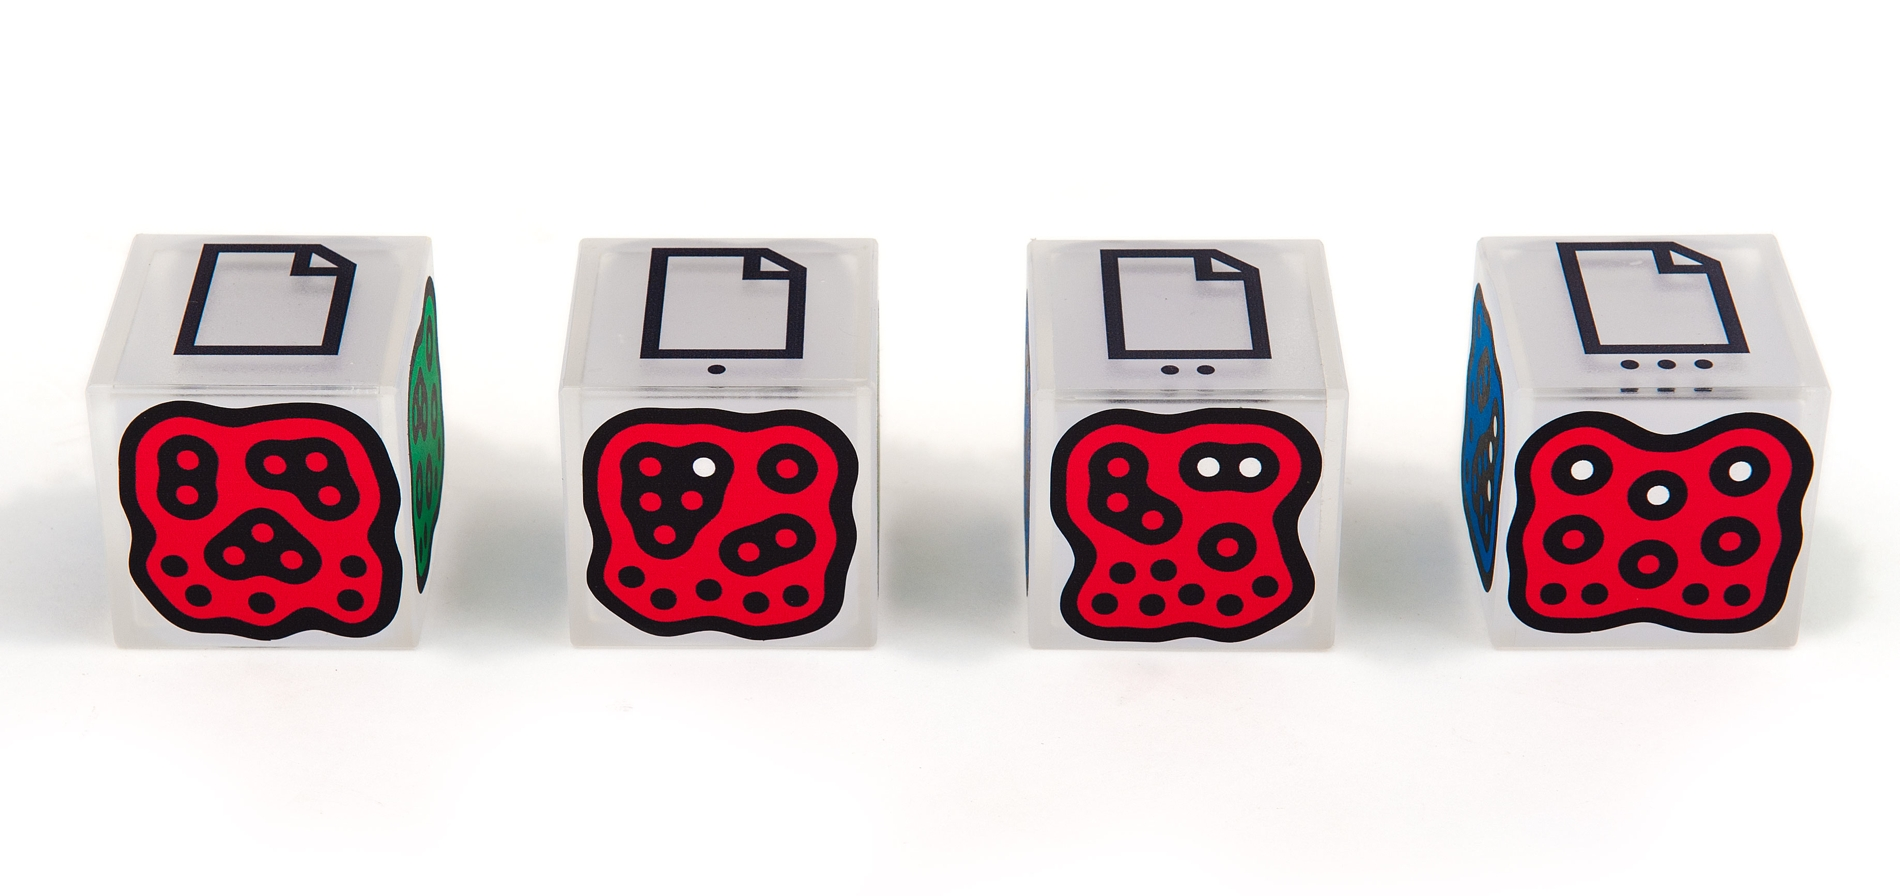
\includegraphics[width=0.6\textwidth]{images/reactelements}
\caption{Élément tangible utilisé pour la génération d'un élément de synthétiseur sur la Reactable\protect\footnotemark}
\label{fig:reactelem}
\end{figure}

\footnotetext{Source: \href{http://a-blok.com/FR/reactable.html}{Reactable : Elements tangibles}}

Chaque élément tangible représente un élément de synthétiseur qu'il est possible de contrôle de plusieurs façon:
\begin{itemize} 
\item La distance de l'élément par rapport a un autre élément. Cette propriété peut être utilisée pour contrôler, par exemple, l'interaction entre deux éléments.
\item L'orientation de l'élément sur la table. Cette propriété peut être utilisé pour contrôler, par exemple, la fréquence de l'élément ce qui va avoir pour effet par exemple pour un battement de ralentir ou d'accélérer ce dernier.
\item La disposition de l'élément. Cette propriété permet entre autre de combiner des éléments pour créer des nouveaux son plus riches et plus complexes.
\item La position du doigt de l'utilisateur par rapport a un élément. On peut venir contrôler divers paramètre comme l'amplitude par exemple en venant faire graviter son doigt autour d'un élément.
\end{itemize}
Ainsi, c'est en combinant plusieurs éléments entre eux avec différentes orientation et différentes dispositions que l'utilisateur va pouvoir peu a peu "construire" sa musique.
Au delà de la détection des éléments tangible, la table est rétro éclairée et permet donc la visualisation en directe de la musique générée (fig.~\ref{fig:reactivsu}).

\begin{figure}[H]
\centering
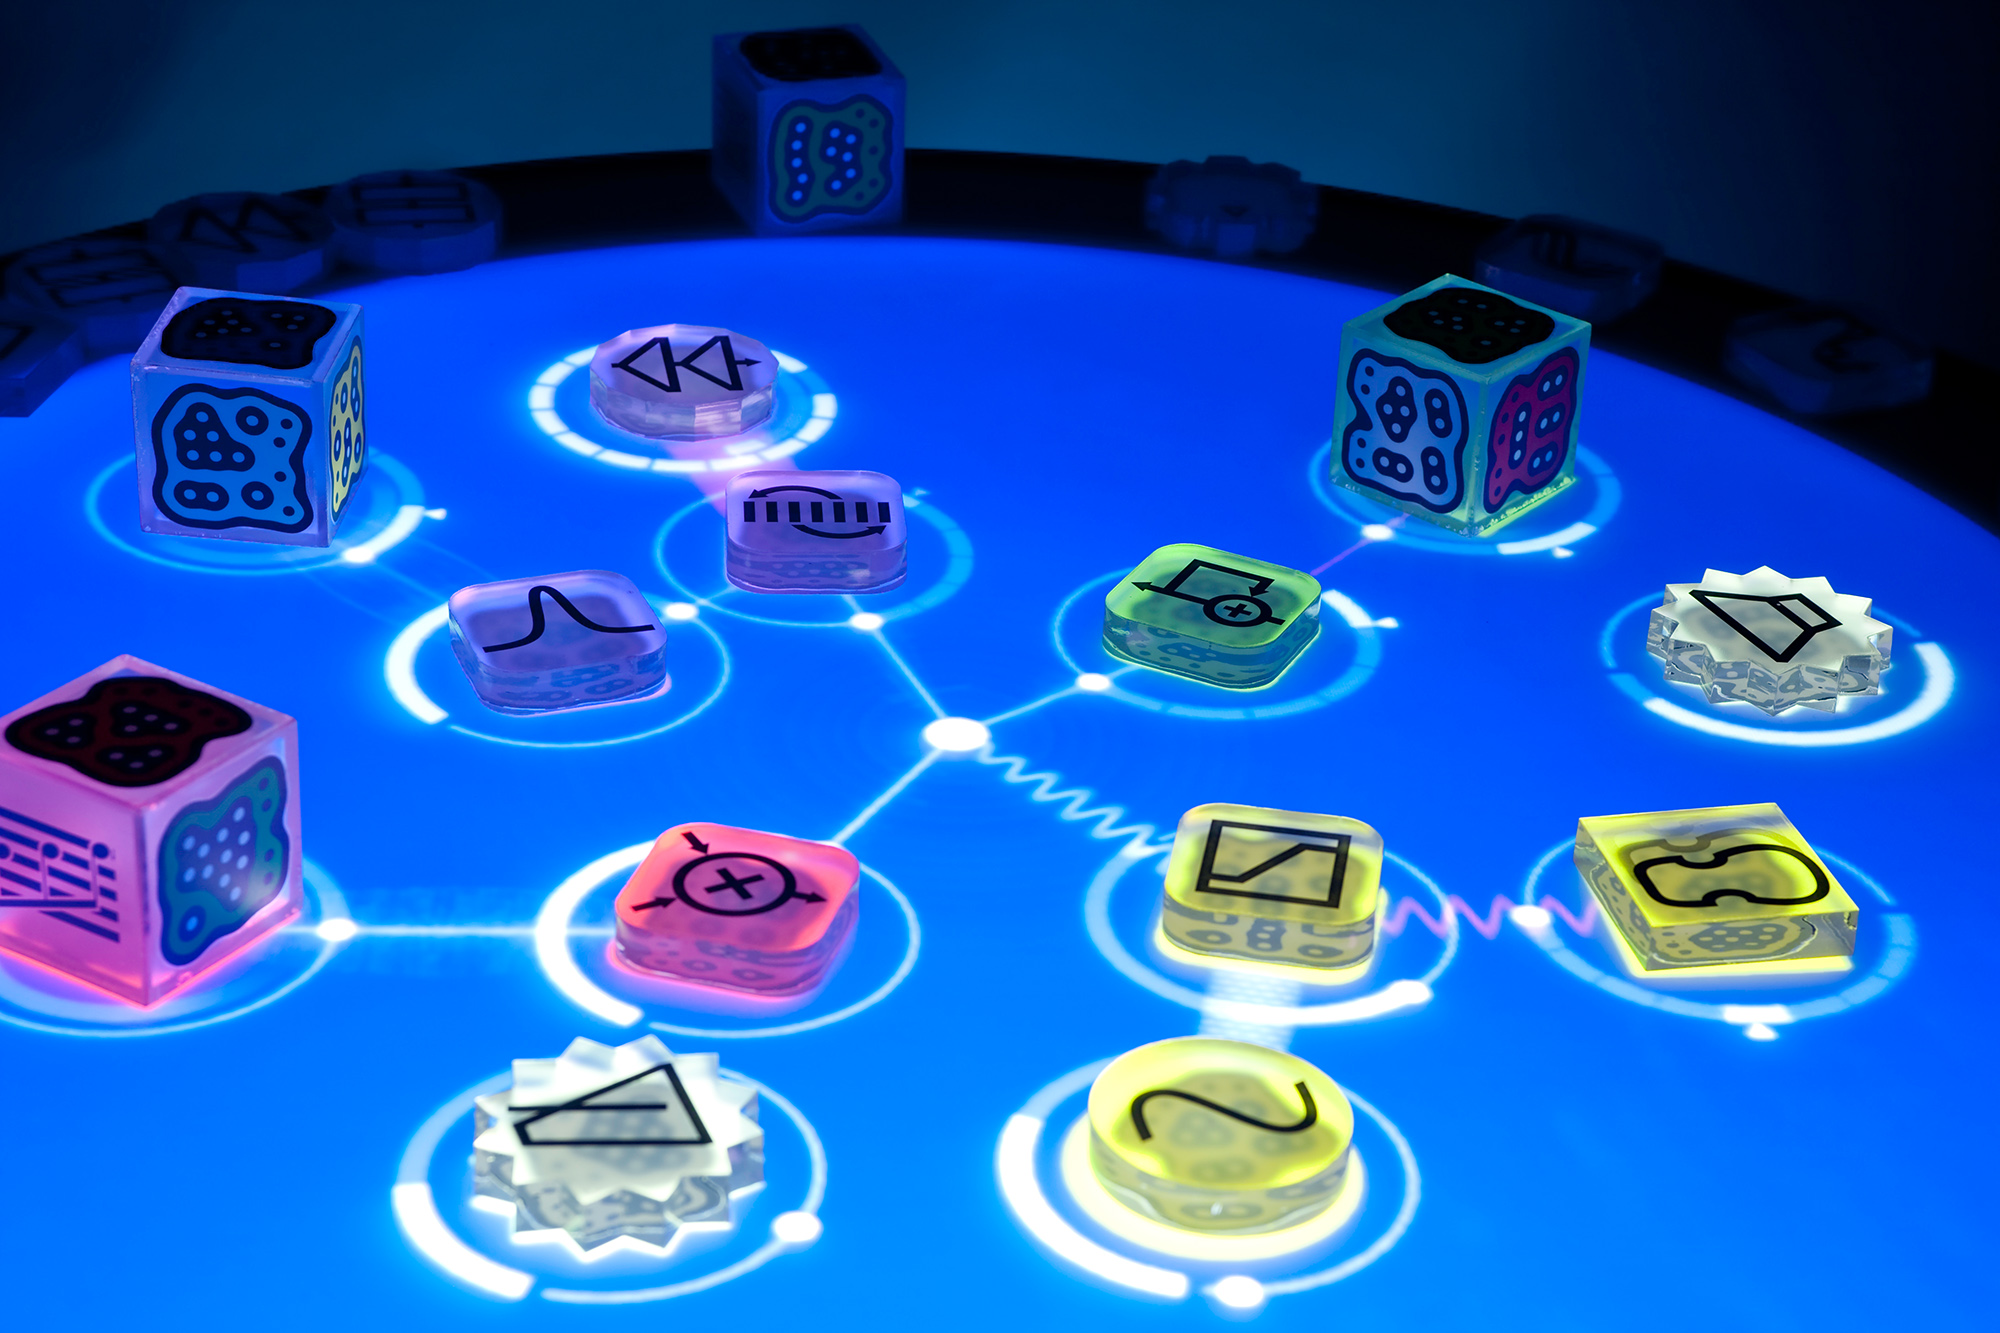
\includegraphics[width=0.65\textwidth]{images/reactvisu}
\caption{Visualisation du son sur la Reactable\protect\footnotemark}
\label{fig:reactivsu}
\end{figure}

\footnotetext{Source: \href{http://a-blok.com/FR/reactable.html}{Reactable}}

\subsection{Besoins de l'application}
\label{subsec:reartable:content}
Le but de l'application était de proposé une démonstration ce de qu'est capable de faire le système proposé par RealityTech et non pas de créer une simulateur de musique en direct fini reprenant tous les points de la Reactable. Un tel développement pourrai faire l'objet d'un stage entier et ce n'était pas le cas ici.

Pour être en adéquation avec l'idéologie de l'entreprise, l'interface tangible et les modes d'interactions avec la musique était le point le plus cruciale. 
En gardant ça en tête nous avons défini les besoins fonctionnels principaux:
\begin{itemize}
\item Générer du son en direct.
\item Créer une représentation physique du son. Chaque son ou élément sonore devait avoir une représentation physique qui lui était associé, c'est à dire, un élément ou groupement d'éléments tangibles représentant ce son.
\item Détecter des éléments physiques représentant les éléments sonores dans une image. L'application devait pouvoir détecter dans une image de caméra les divers éléments physiques présents de façon a ce qu'ils soient utilisés pour identifier les éléments sonores.
\item Identifier les représentation physique des sons. Chaque élément sonore étant représenter par un ou plusieurs éléments physique, l'application devait être capable, à partir des résultats de la détection, d'identifier et de différencier des éléments sonores entre eux. 
\item Modifier un élément sonore. L'application devait pouvoir contrôler certains paramètre défini a l'avance de chaque élément sonore généré. Ces paramètres ont pour but d'apporter a l'utilisateur a un niveau de contrôle supérieur lors de la création de musique en direct.
\item Détecter des événements liés au toucher. Dans le cas du contrôle d'un son, l'utilisateur peut être amener a toucher des zones interactives pour déclencher divers effets.
\item Créer une visualisation basique d'un son. L'application devait proposer une visualisation du son généré pour guider l'utilisateur dans son expérimentation.
\end{itemize}

\subsection{Choix et implémentation}
\label{subsec:reartable:impl}
L'application a donc été développé avec Processing en utilisant PapARt pour la partie visualisation, détection et projection et Sonic Pi\cite{sonicpi} pour la génération de musique en direct.
Sonic Pi est un synthétiseur temps réel qui permet très facilement de générer des sons de manière cohérente. Le gros avantage de Sonic Pi est qu'il résout tout seul énormément de problèmes posé par la génération dynamique de musique comme par exemple la synchronisation des boucles, les effets d'entrée et de sortie des instruments et bien d'autre ce qui dé-complexifie énormément le processus.

Comme on peut le voir sur le schéma explicatif (fig ~\ref{fig:reartable:generalscheme}), les éléments tangibles représentants des sons se présentent sous forme de regroupement d'éléments rond de petite taille (des aimants dans notre cas). L'idée derrière ce choix est d'encourager la manipulation d'élément physique pour garder le contenu numérique en contexte et favoriser la création. On peut différencier deux sons en fonction du contenu du regroupement (nombre, position et couleur des éléments regroupés).

\begin{figure}[H]
\centering
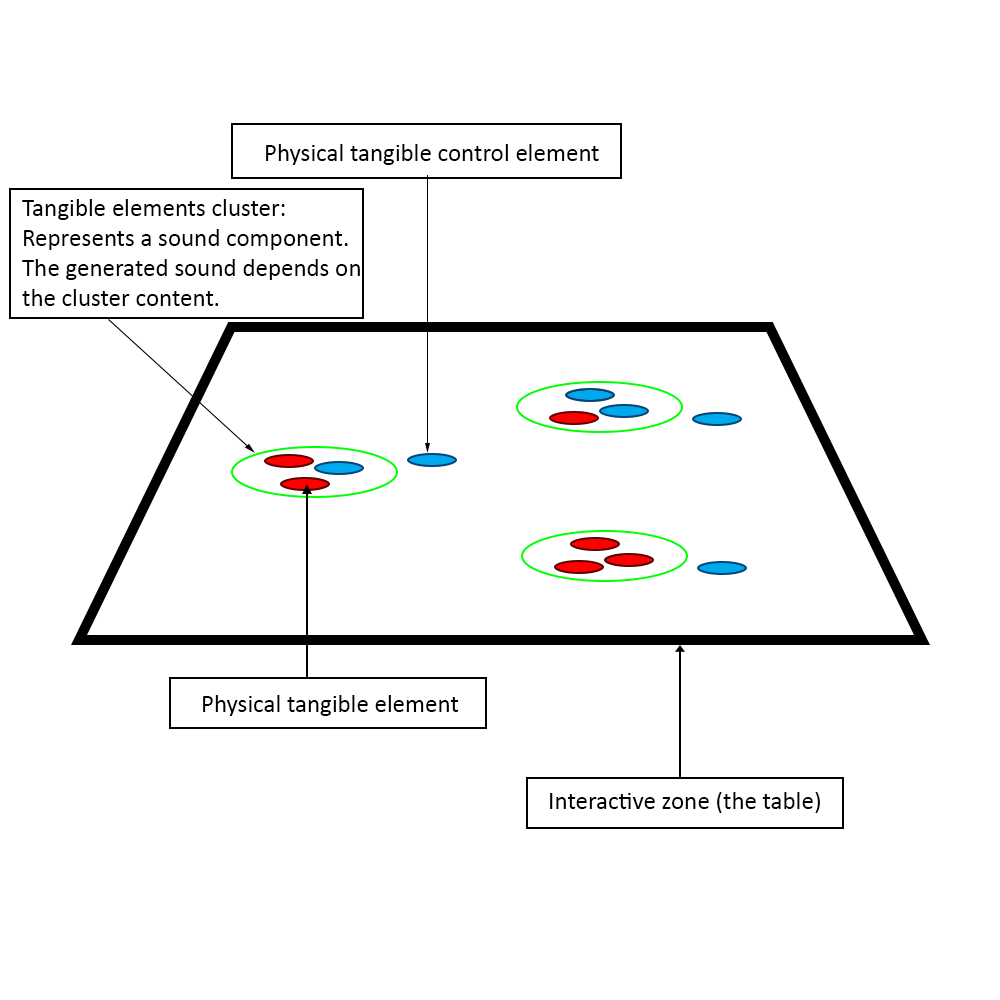
\includegraphics[width=0.5\linewidth]{images/rearproto}
\caption{ReARtable: Schéma général}
\label{fig:reartable:generalscheme}
\end{figure}

Une fois les éléments détectés, regroupés et identifiés, l'élément sonore associé peut être créer. La création d'élément sonore se fait simplement via la transmission d'un message OSC\footnote{Le protocole OSC où OpenSoundControl est un format de transmission de donnée conçu pour le contrôle en temps réel} à un serveur Sonic Pi préalablement démarré. Ce message contient l'identifiant unique de la boucle que Sonic Pi doit démarrer. Pour chaque éléments sonores que l'application peut créer Sonic Pi possède une fonction a exécuter que nous avons préalablement créer. Toutes les communications entre l'application et Sonic Pi utilisent ce protocole ce qui permet de démarrer/arrêter/modifier certaines partie du son en directe.

Pour ce qui est du contrôle du son, une zone autour du composant est défini dans laquelle soit un élément tangible, soit une interaction physique (avec le doigt) vont être détecté et converti en interaction avec le contenu numérique (fig.~\ref{fig:reartable:interactionzone}).

\begin{figure}[H]
\centering
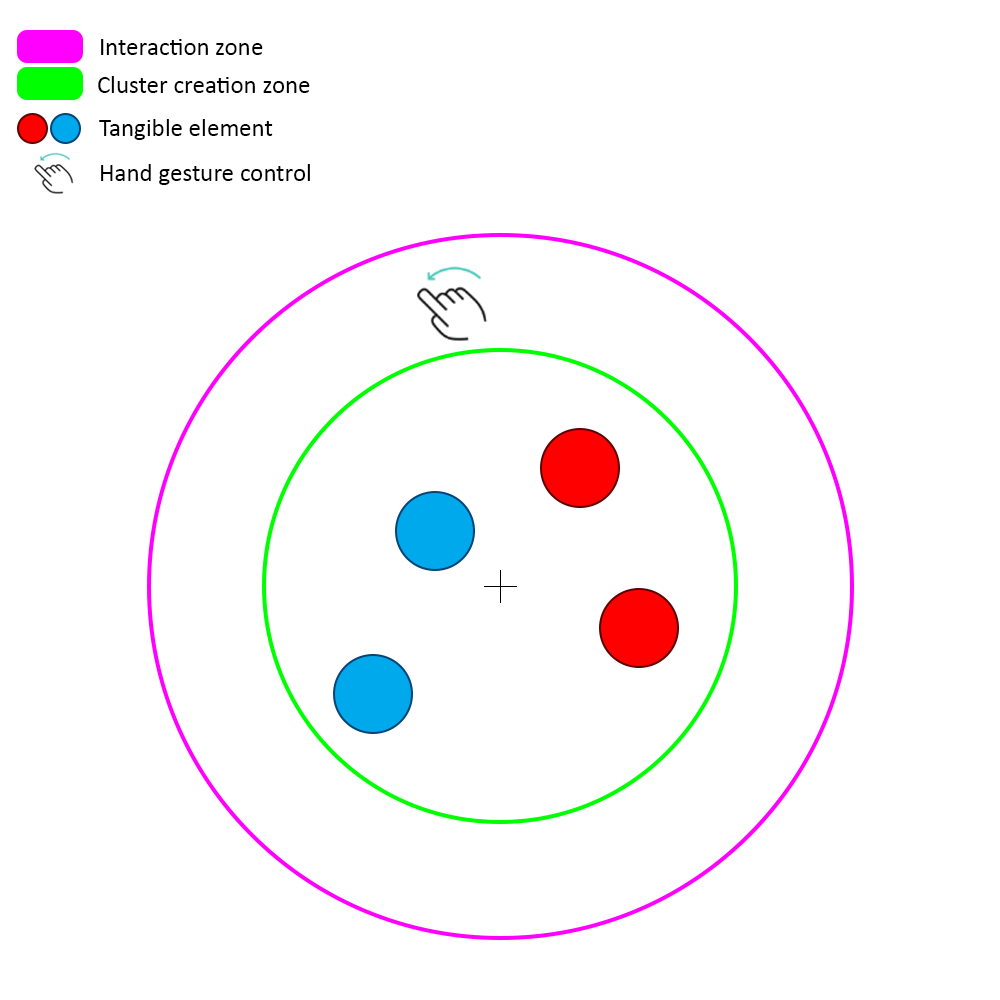
\includegraphics[width=0.45\textwidth]{images/reartable_cluster_interaction}
\caption{Schéma représentant la création d'un son avec zone d'interaction}
\label{fig:reartable:interactionzone}
\end{figure}

La dernière étape du développement de l'application était la visualisation de la musique générée (section ~\ref{subsec:reartable:content}). Cette étape n'a finalement pas été abouti par manque de temps. L'idée était d'utiliser le spectre du son et les différentes fréquences qui le compose récupérable a l'aide d'une transformée de fourrier\footnote{Opération mathématique permettant de décomposer un signal en la somme des signaux qui le compose \href{https://fr.wikipedia.org/wiki/Transformation_de_Fourier}{Wikipédia - Transformation de Fourier}.} pour créer une visualisation globale basée sur les fréquences avec des variations visuels en fonction de la hauteur, du tempo du son et tous les autres paramètre du son qu'on peu extraire.

\begin{figure}[H]
\centering
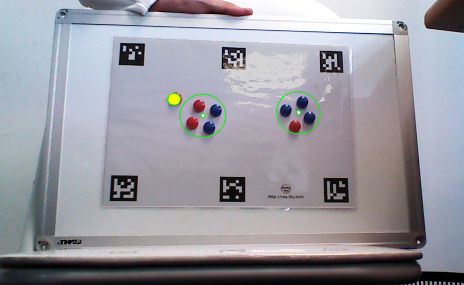
\includegraphics[width=0.65\linewidth]{images/reartable}
\caption{Démonstration de l'application}
\label{fig:reartable:demo}
\end{figure}

\newpage
\section{Extraction de document}
\label{sec:document}
Plus tard au cours de mon stage des cas d'utilisation où l'extraction et la numérisation de document ont été abordé comme par exemple l'écriture d'une lettre en réalité augmentée et ainsi il était judicieux de développer une preuve de concept de cette fonctionnalité sous la forme d'une application de SAR.

Le but de ce développement était d'expérimenter diverses techniques de détection de document en temps réel se basant ou non sur des connaissances à priori comme la taille du document, sa couleur, la couleur du fond (duquel il falloir extraire le document), la présence d’éléments distinctifs (comme des marqueurs fiduciaires ou des ronds colorés de petite taille).

\subsection{Besoins de l'application}
\label{subsec:doc:content}
\begin{itemize}
\item Accéder au flux vidéo d'une caméra. L'application devait avoir access au flux vidéo d'une caméra filmant le document à détecter.
\item Détecter un document dans une image. Des images extraites du flux vidéo, l'application devait être capable, avec ou sans connaissance a priori, de détecter un document se trouvant dans cette image.
\item Extraire un document d'une image. Grâce au résultat de la détection, l'application devait être capable d'extraire ce document de l'image afin d'obtenir une image ne contenant que le dit document.
\end{itemize}

\subsection{Choix et implémentation}
\label{subsec:doc:impl}

La détection de document est un problème connu en traitement d'image sur lequel j'avais déjà eu l'occasion de travailler lors de mon projet de fin d'études durant le deuxième semestre de mon année de Master 2.

Dans cette application nous avons mis en place plusieurs détection différentes pour essayer de trouver une solution a ce problème.

\paragraph{Détection de document basé sur des marqueurs colorés} La première détection utilise une connaissance a priori sur le document: Le document cible est muni de lignes d'éléments ronds colorés de petite taille dans un ou plusieurs de ses coins (fig. ~\ref{sub:doc}). Ainsi tout l'enjeu de cette détection se base dans la détection de ces éléments colorés dont il est question plus tard dans ce rapport (voir section ~\ref{sec:sticker-detection}).

Une fois les éléments détectés, ils sont regroupés en différentes lignes (fig. ~\ref{sub:docline}).
Une ligne est défini par un regroupement d'éléments dont l'écart entre chaque éléments ne dépasse pas une certaine distance verticale ou horizontale. L'angle de la ligne est défini par les deux premiers éléments qui la compose. Si un autre élément "dérive" il est rejeté et la ligne est créée. Cette ligne est ensuite utilisé pour calculer deux vecteurs, dont un est confondu avec la ligne et le deuxième est perpendiculaire au premier (fig ~\ref{sub:doclineperp}).
La détection finale du document se fait en calculant l'intersection des différents vecteurs verticaux et horizontaux (fig. ~\ref{sub:docextract})

\begin{figure}[H]
    \centering
	\subfloat[Document marqué à détecter]{
      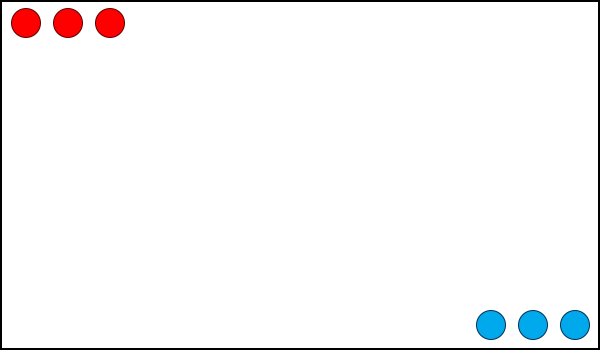
\includegraphics[width=0.45\textwidth]{images/document}
      \label{sub:doc}
      }
    \subfloat[Détection des éléments rond et création des lignes]{
      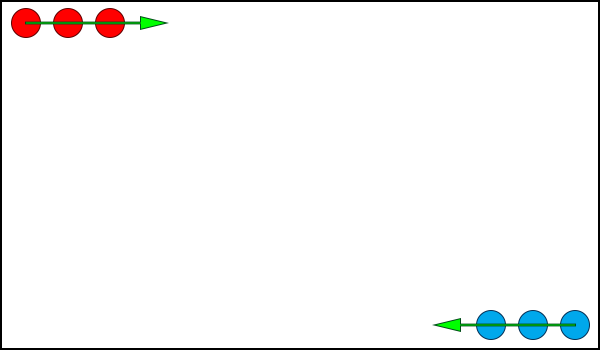
\includegraphics[width=0.45\textwidth]{images/doc-line}
      \label{sub:docline}
      }
      \\
      \subfloat[Génération des information manquante pour finaliser la détection]{
      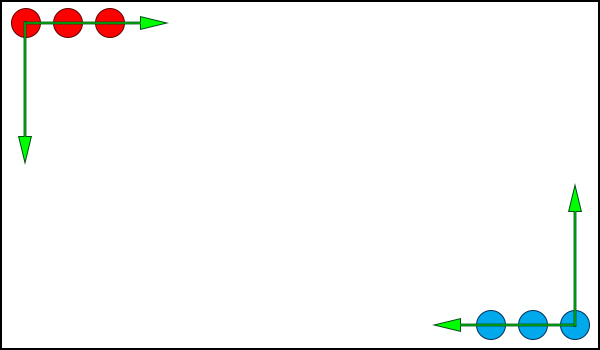
\includegraphics[width=0.45\textwidth]{images/doc-line-perp}
      \label{sub:doclineperp}
      }
    \subfloat[Document détecté]{
      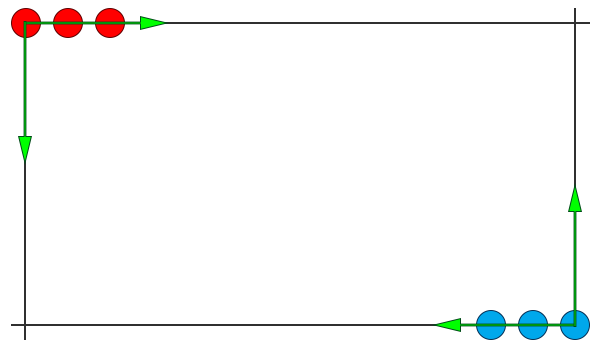
\includegraphics[width=0.45\textwidth]{images/doc-extraction}
      \label{sub:docextract}
      }
\caption{Détection de document étape par étape}
\label{fig:docdetection}
\end{figure}

Comme on peut le voir figure ~\ref{sub:docextract}, lors de cette détection les bords du document sont rognés. Généralement ces zones ne contiennent aucune information car elles correspondent généralement aux marges verticales et horizontales que chaque document possède. Cependant comme évoqué dans les cas d'utilisation, cette détection ne sera pas utiliser seulement pour des documents de type A4, on pourra s'en servir comme outil pour suivre une feuille de papier a la manière des marqueurs ARToolKit, ou pour détecter des post-it par exemple. Ainsi ces marges ne peuvent pas être ignoré dans notre cas.

Une simple connaissance a priori de la distance des éléments rond par rapport au coin permet de résoudre ce problème ou alors pour avoir une détection bien plus précise et robuste, il est possible d'utiliser des algorithmes de détection de contour couplé a des algorithmes d'extraction de lignes pour retrouver le vrai coin du document. C'est ce dont nous allons parler dans la deuxième partie.

\paragraph{Détection de document - Canny et transformée de Hough} Sans connaissance a priori la détection de document devient un problème compliqué et bien connu du monde de l'informatique surtout lorsqu'il un besoin de temps réel vient s'ajouter la tâche, comme par exemple, dans une application de scan de document.

L'algorithme de Canny\cite{Canny86acomputational} est un filtre de détection de contour permettant d'extraire d'une image des contours (fig ~\ref{sub:detectedge}) très précis respectant trois critères : La bonne détection, la bonne localisation et la clarté de la réponse. Ces trois critères en font un très bon choix dans le cadre de la détection de document ou la qualité et surtout la précision de la détection est importante pour ne pas rogner des bouts de document par exemple. Cet algorithme a cependant tendance à laisser beaucoup de bruit issue de faible contour tout de même détectés c'est pourquoi il faut effectuer une étape de floutage préalable afin de lisser les zones a faible contour.

Une fois les contours détectés, il est possible d'essayer d'extraire directement le document mais c'est une tâche plus complexe, car elle requiert d'analyser les contours, qu'il est possible de facilité en utilisant la transformée de Hough\cite{hough}. La transformée de Hough permet d'extraire n'importe quelle forme a partir d'une image contour en utilisant les propriété mathématiques de la forme. Dans notre cas où nous souhaitons extraire des lignes droites les propriétés mathématiques utilisés correspondent aux coordonnées polaires considérés comme plus robuste que l’équation de la droite (fig ~\ref{sub:detectline})

\begin{figure}[H]
\centering
	\subfloat[Image originale\protect\footnotemark]{
      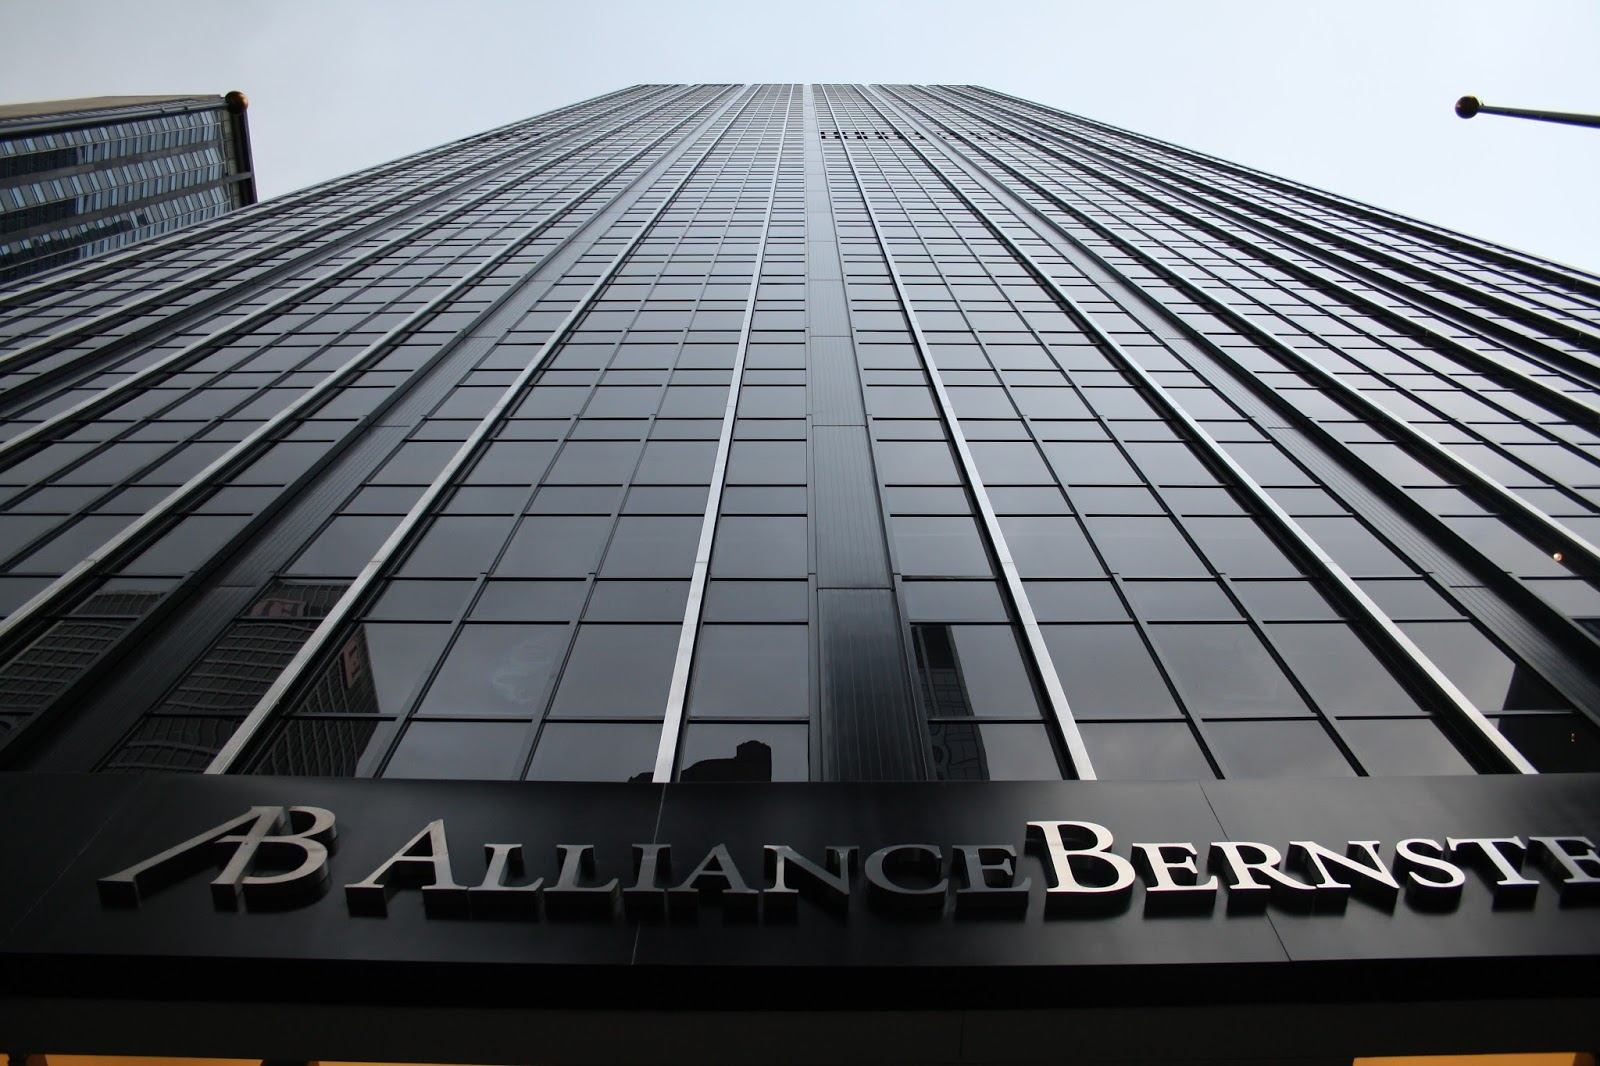
\includegraphics[width=0.45\textwidth]{images/detection-original-image}
      \label{sub:originalimage}
      }
      \\
	\subfloat[Canny - Détection de contours\protect\footnotemark]{
      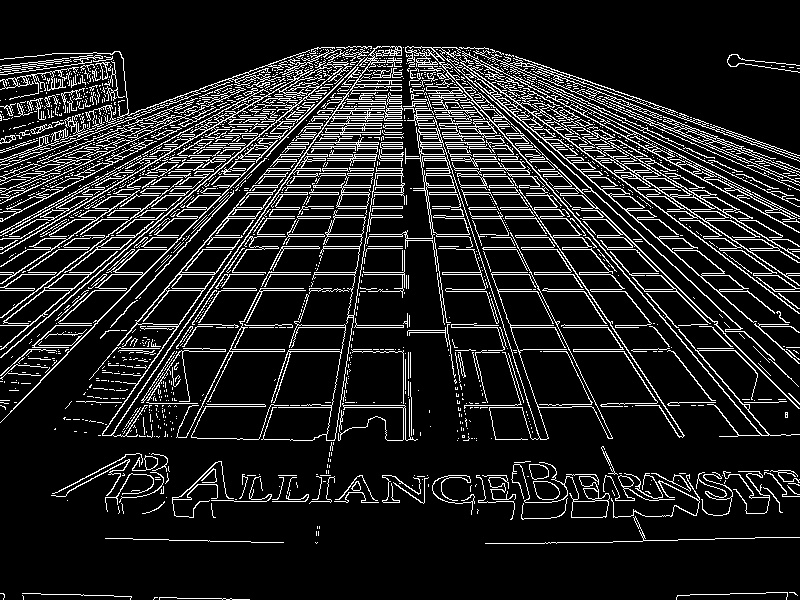
\includegraphics[width=0.45\textwidth]{images/cannysample}
      \label{sub:detectedge}
      }
    \subfloat[Transformée de Hough - Détection de lignes\protect\footnotemark]{
      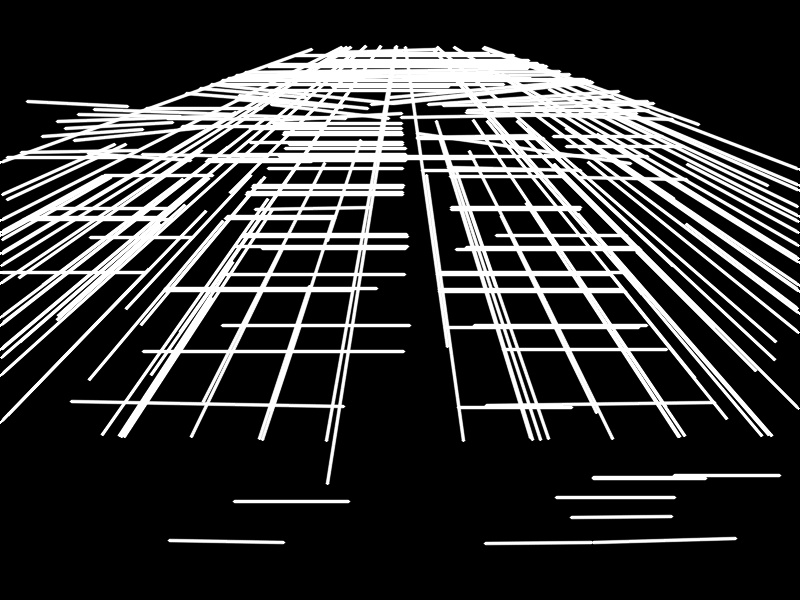
\includegraphics[width=0.45\textwidth]{images/houghsample}
      \label{sub:detectline}
      }
\caption{Détection de lignes : Canny + Hough }
\label{fig:cannyhough}
\end{figure}
\footnotetext{Source : \href{http://funvision.blogspot.com/2016/01/hough-lines-and-canny-edge-sobel.html}{http://funvision.blogspot.com/2016/01/hough-lines-and-canny-edge-sobel.html}}
\footnotetext{Source : \href{http://funvision.blogspot.com/2016/01/hough-lines-and-canny-edge-sobel.html}{http://funvision.blogspot.com/2016/01/hough-lines-and-canny-edge-sobel.html}}
\footnotetext{Source : \href{http://funvision.blogspot.com/2016/01/hough-lines-and-canny-edge-sobel.html}{http://funvision.blogspot.com/2016/01/hough-lines-and-canny-edge-sobel.html}}

Il ne reste qu'a filtrer les lignes pour trouver des potentiels documents dans une image.

Cette succession de traitement est cependant lourde et peut difficilement être effectué en temps réel sur des images de haute résolution. 
Dans notre cas, nous nous somme servit de ces algorithmes seulement sur des parties d'image (de petite résolution) de façon à améliorer une première détection grossière effectué par exemple, a l'aide de marqueurs colorés. Une fois la première détection effectué, nous obtenons une position plus ou moins précise des quatre coins nécessaire à l'extraction du document.
Nous utilisons cette information sur la position potentiel des coins pour extraire dans des sous image centrés sur ces coins (fig. ~\ref{sub:subimage:subimage}). Ensuite nous appliquons les deux algorithmes mentionné plus tôt, a savoir, la détection de contour (fig. ~\ref{sub:subimage:canny}) puis la détection de ligne (fig. ~\ref{sub:subimage:hough}). Nous filtrons ensuite le résultat de la détection de ligne pour obtenir exactement une ligne vertical et une ligne horizontale. Une fois ces deux lignes trouvés, nous calculons les équations de droite (pente, et constante) associés pour pouvoir en calculer l'intersection et finalement trouver le coin dans cette sous image (fig ~\ref{sub:subimage:corner}).

\begin{figure}[H]
\centering
	\subfloat[Sous image autour d'un coin.]{
      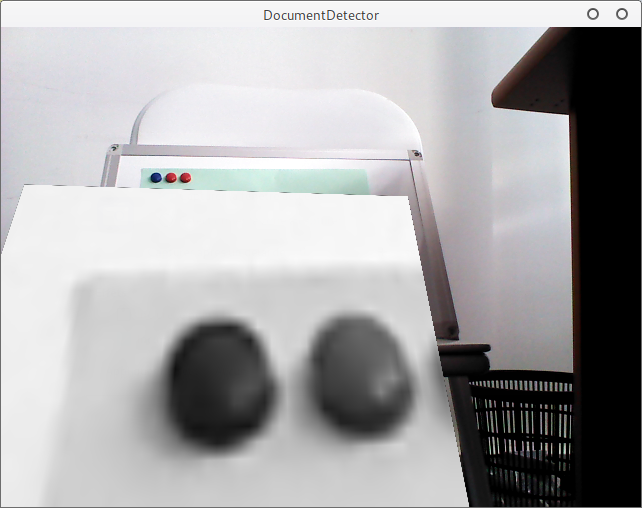
\includegraphics[width=0.45\textwidth]{images/image-original-corner}
      \label{sub:subimage:subimage}
      }
    \subfloat[Canny - Détection de contour basée sur un seuillage de l'image originale]{
      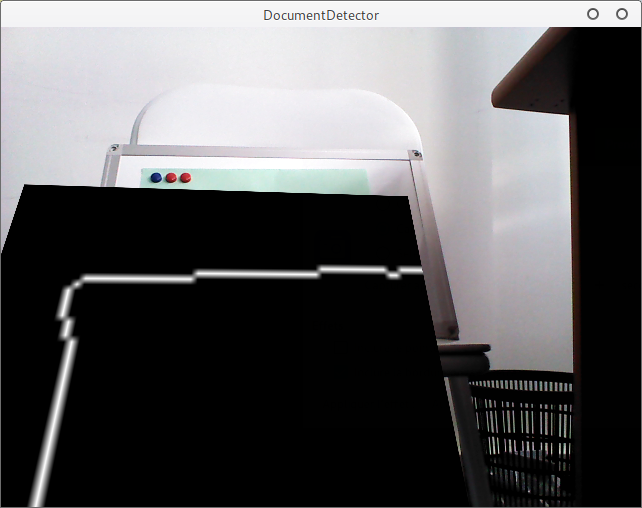
\includegraphics[width=0.45\textwidth]{images/canny-corner}
      \label{sub:subimage:canny}
      }
      \\
	\subfloat[Hough - Détection de lignes basée sur le résultat de Canny]{
      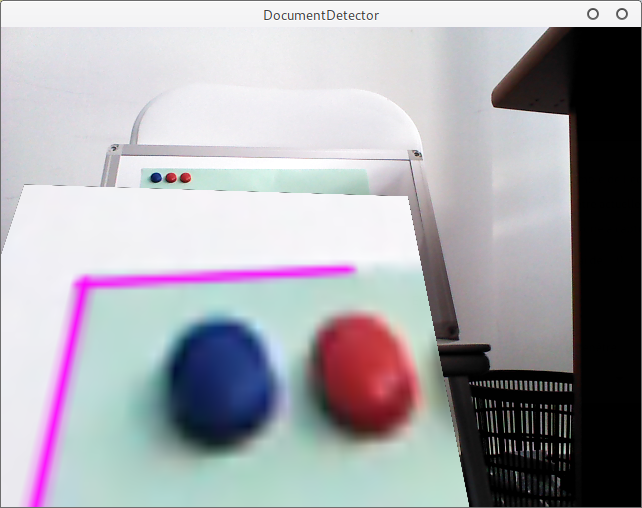
\includegraphics[width=0.45\textwidth]{images/hough-corner}
      \label{sub:subimage:hough}
      }
    \subfloat[Détection finale du coin.]{
      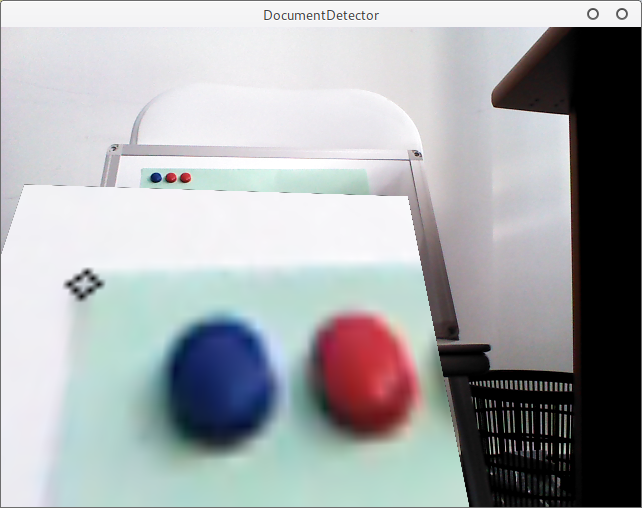
\includegraphics[width=0.45\textwidth]{images/corner-corner}
      \label{sub:subimage:corner}
      }
\caption{Affinage de la détection d'un coin du document}
\label{fig:corner-redetect}
\end{figure}

\paragraph{Bilan}
Pour finir, vous trouverez Figure %TODO 
un rapide comparatif des différents résultats obtenus. On peut observer quelques points notables : En utilisant Hough et Canny pour améliorer la détection d'un coin, l'extraction est plus fidèle au document réel. En effet, les coins détectés sont plus précis que des hypothèses effectués à priori. Cette méthode est cependant moins rapide car elle requiert de nombreux calculs en plus. Lorsque utilisé en temps réel, on peut cependant observer que la détection avec connaissance à priori du modèle est bien plus robuste, car elle ne dépend pas d'une deuxième détection qui a beaucoup de chance d'échouer (seuillage, détection de contour, détection de ligne, intersection entre deux droites puis obtention finale du coin) ainsi la méthode a utiliser variera avec les cas d'utilisations. Par exemple dans le cadre d'une application de scan de document, une méthode d'extraction de document plus précise sera envisagée, mais dans le cadre d'une estimation de pose il sera préférable d'utiliser une détection rapide et robuste.
